

\section{「滞在ウォッチ」のシステム構成}\label{3.1}



% 本研究のシステム概要を図\ref{StayWatchOverview}に示す.
「滞在ウォッチ」は利用者がビーコンを携帯し,部屋ごとに設置された受信機によりビーコンを検出する手法で,在室者管理を自動に行う.
部屋利用者には一人1つビーコンを携帯してもらう.
サーバには部屋利用者の名前とビーコンのIDを登録する.
ビーコンは周囲に数秒に1回電波を発信する.
受信機がビーコンの電波を受信する間隔は3分である.
受信機が検出したビーコンのIDと電波強度はサーバに送信され,日時と在室した部屋名が記録される.
記録した在室者情報はWeb APIを通して利用可能であり,勤怠管理システムや来訪促進システムといった様々な応用を想定している.

\begin{figure}[h]
  \centering  % 図を真ん中に配置
  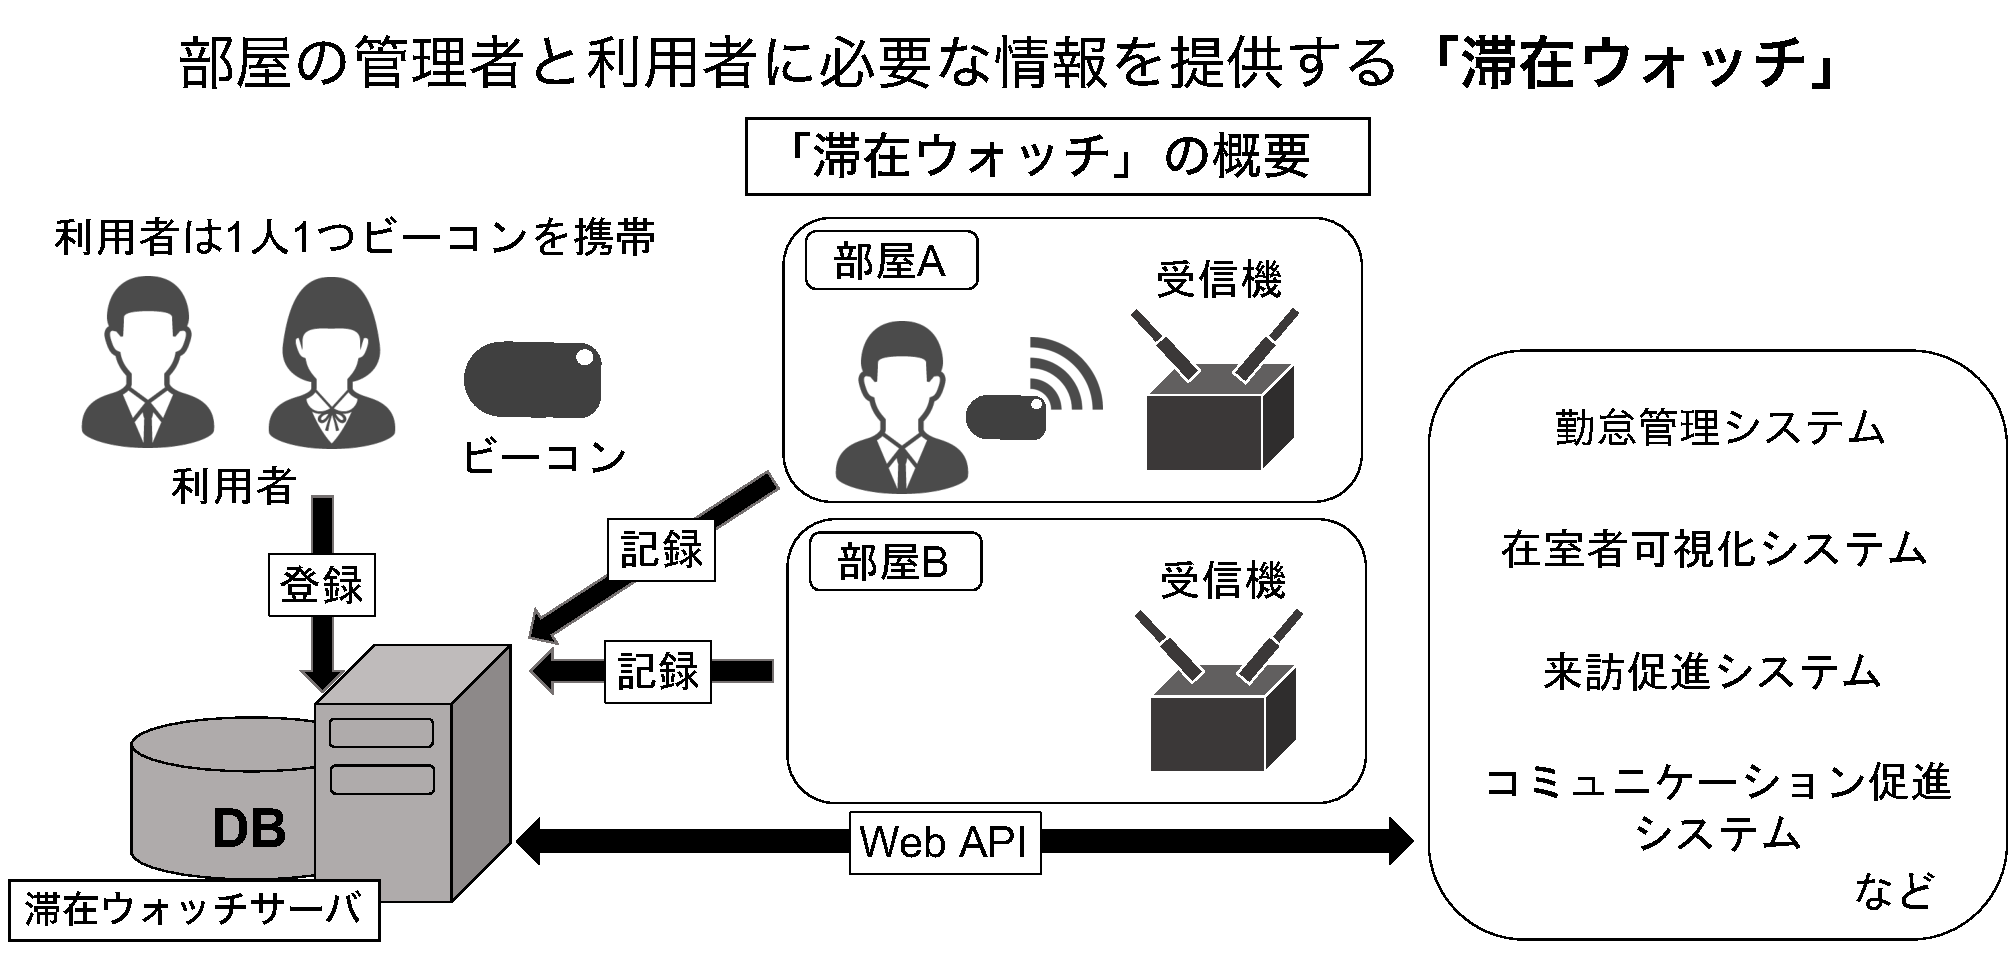
\includegraphics[clip,scale = 0.45]{image/platform-idea.pdf}
  \caption{「滞在ウォッチ」の概要図}    \label{StayWatchOverview}
\end{figure}

本手法に関連するビーコン,受信機,サーバを示す.
利用者が携帯するビーコンには,長期的な運用を考慮し電池交換が可能かつ小型なFCS1301\cite{fcs1301}を利用している.
ビーコンは図\ref{fig:beacons}のように様々な大きさや形のものがある.
複数のビーコンの比較を表\ref{tb:beacons}に示す.
ボタンは定期的な電波発信に加えて押した時にも電波発信できるため,点検時に利用できる.
FCS1301の用途は,財布やパスケースなどの貴重品に付ける紛失防止や子供の荷物などに付ける見守り支援がある.
実際にパスケースに取り付けた様子を図\ref{fig:beaconforpass}に示す.
財布やパスケースに取り付けたり入れても気にならないサイズだとわかる.
そのため,利用者が携帯するのに適している.
また電池交換の際の様子を図\ref{fig:batchange}に示す.
特殊な器具などを使う必要がなく,簡単に電池交換ができる.
FCS1301ではボタンを押すとペアリング,長押しするとスリープモードへ移行し,保管の間省電力モードになる.
ビーコンの電波送信の間隔はFCS1301の規格で最大の10秒ごとに設定している.
部屋ごと設置する受信機には図\ref{fig:raspi}の低価格なRaspberry Pi\cite{raspi}を利用している.
1つの部屋に1つずつ受信機を設置する.
サーバには,Google Cloud Platform\cite{platform}を利用している.

% \begin{figure}[H]
%   \begin{center}
%     \includegraphics[width=150mm]{image/BeaconType.png}
%     \caption{ビーコンの種類}
%     \label{fig:beacons}
%   \end{center}
% \end{figure}

% \begin{table}[H]
%   \begin{center}
%     \caption{ビーコンの比較}
%     \label{tb:beacons}
%     \begin{tabular}{|l|c|c|c|} \hline
%       ビーコン名 & サイズ                            & 電池交換 & ボタン \\ \hline \hline
%       FCS1301    & 縦46.0 mm× 横24.5 mm× 厚さ3.5 mm  & ○        & ○      \\
%       MAMORIO    & 縦35.5 mm× 横19.0 mm× 厚さ3.4 mm  & ×        & ×      \\
%       WICED      & 縦60.0 mm× 横37.0 mm× 厚さ10.0 mm & ○        & ○      \\
%       estimote   & 縦55.0 mm× 横38.0 mm× 厚さ15.0 mm & ×        & ×      \\\hline
%     \end{tabular}
%   \end{center}
% \end{table}

% \begin{figure}[H]
%   \begin{center}
%     \includegraphics[width=150mm]{image/beaconforpass.png}
%     \caption{パスケースに取り付けたビーコン}
%     \label{fig:beaconforpass}
%   \end{center}
% \end{figure}

% \begin{figure}[H]
%   \begin{center}
%     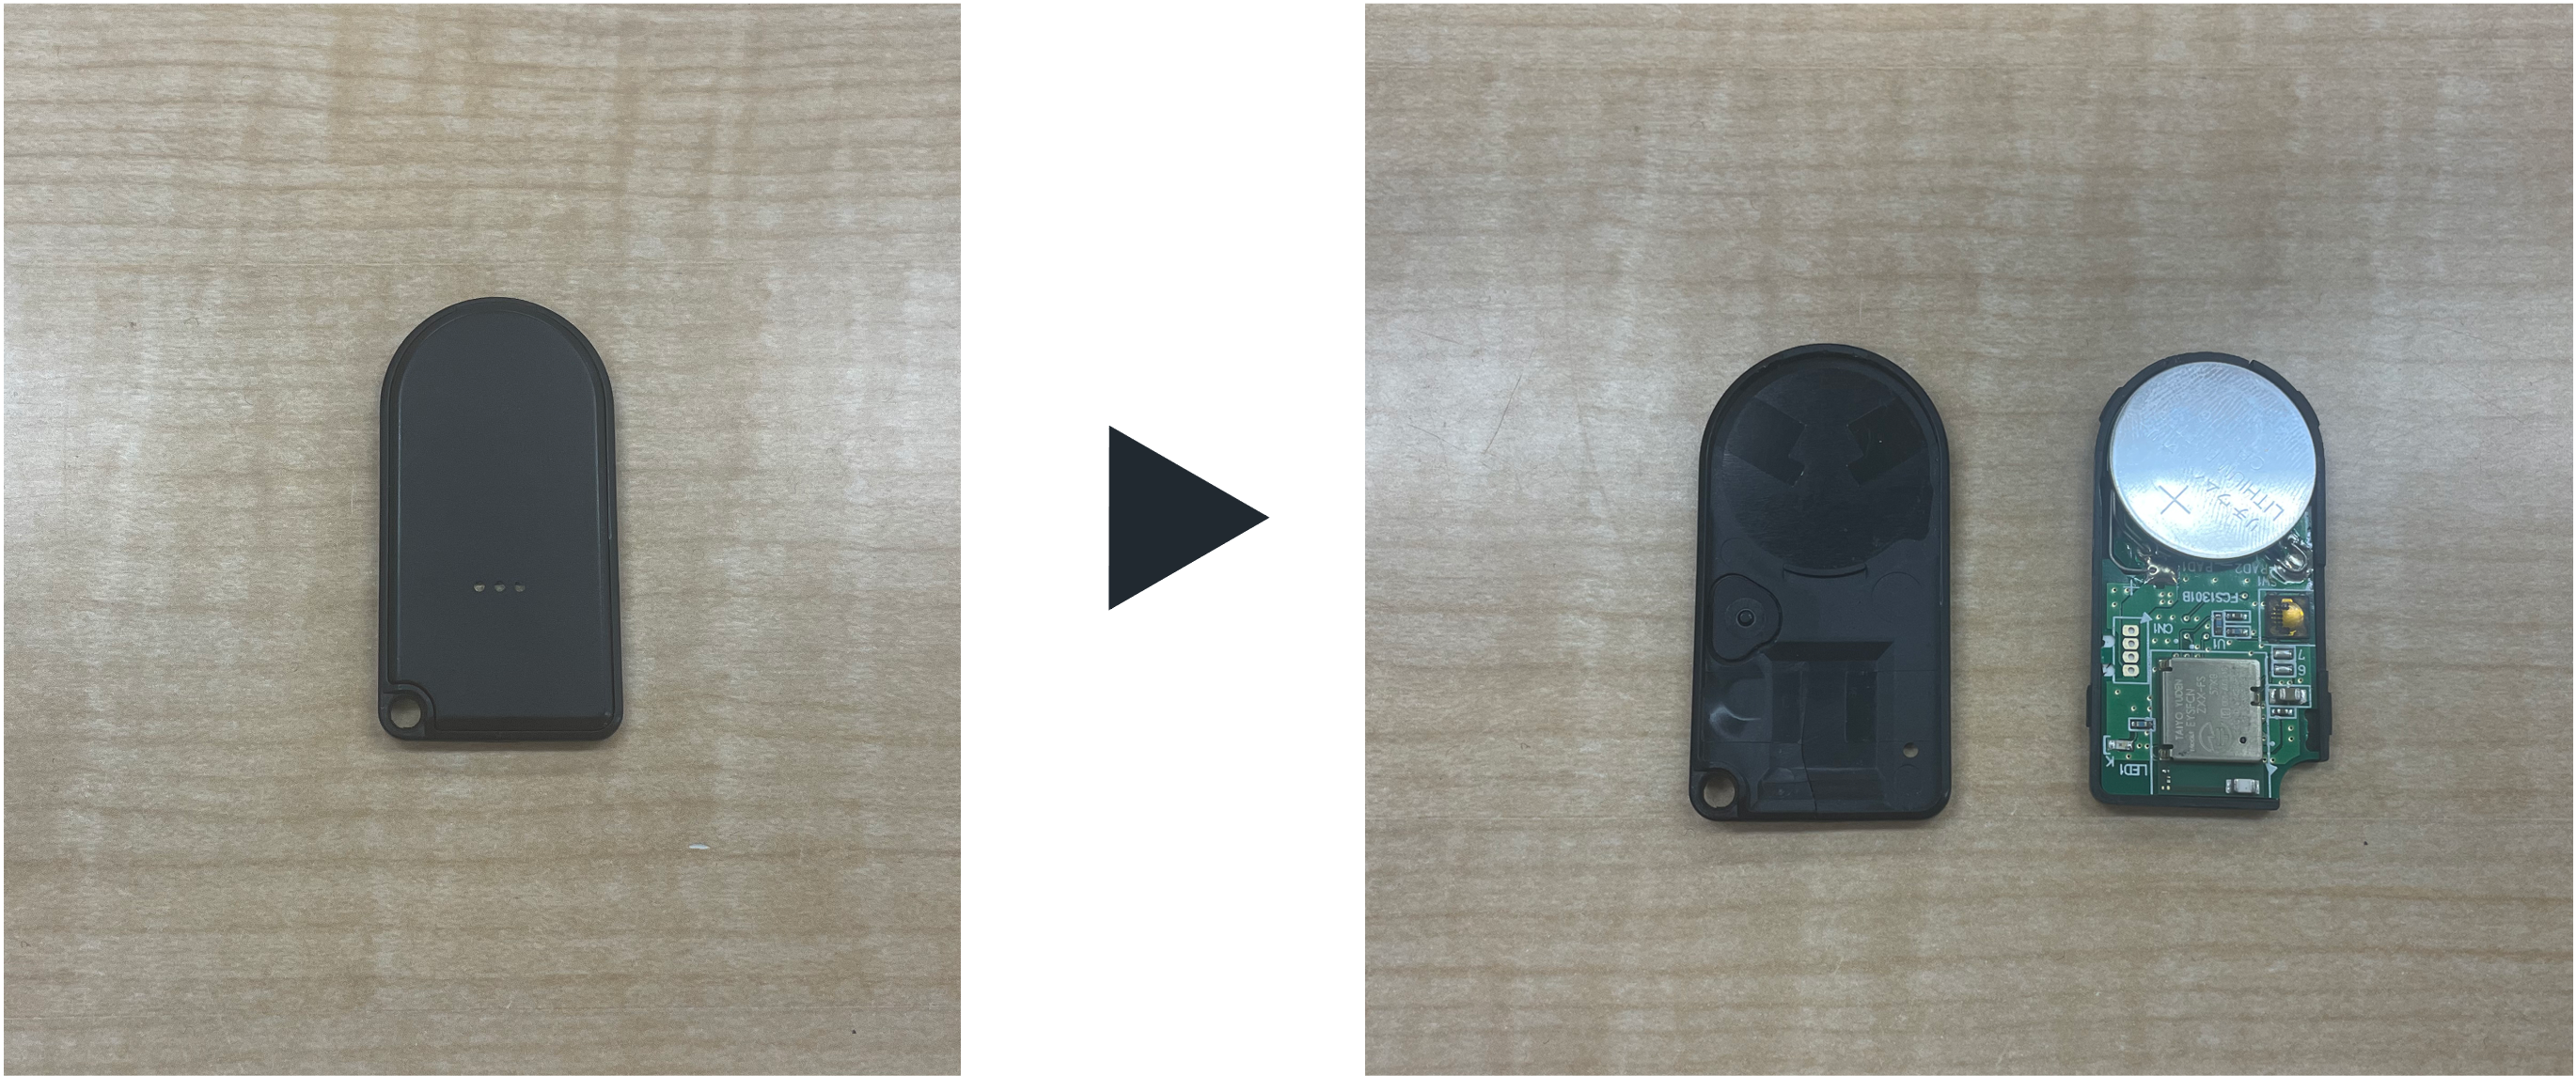
\includegraphics[width=150mm]{image/batchange.png}
%     \caption{ビーコンの電池交換}
%     \label{fig:batchange}
%   \end{center}
% \end{figure}

% \begin{figure}[H]
%   \begin{center}
%     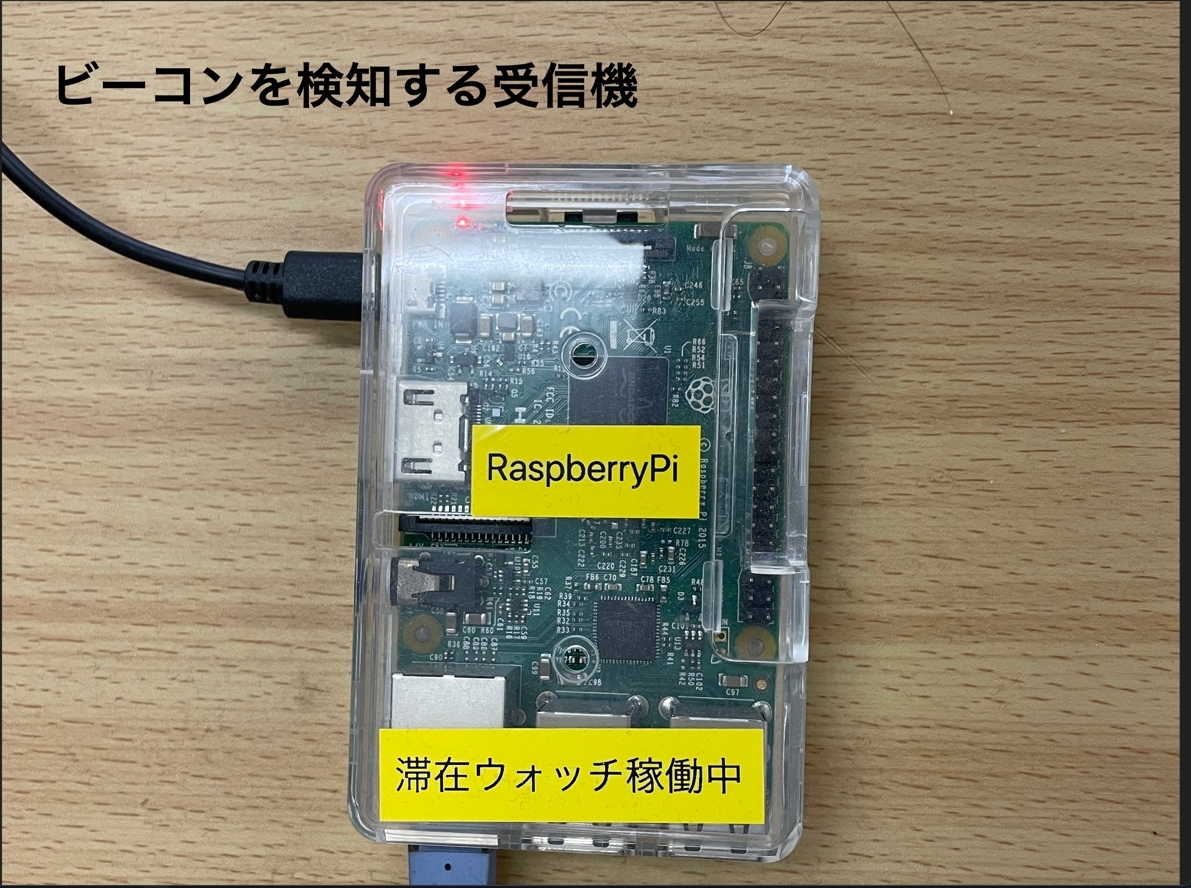
\includegraphics[width=150mm]{image/RasPi.png}
%     \caption{実際に使用しているビーコンを検知する受信機}
%     \label{fig:raspi}
%   \end{center}
% \end{figure}

% 個人を特定する在室者の検出手法には,個人と在室者情報を紐付けする必要がある.
% ビーコンを用いた検出手法ではビーコンのIDと利用者の名前をサーバのデータベースに登録している.
% 登録には図\ref{fig:ent}のウェブサイトを用いて行う.
% グループ分けとして研究室やチームの属性を追加している.
% これは可視化において個人の識別を容易にし,来訪促進システムでは連帯感や競争心を刺激でき,ゲーミフィケーション\cite{gamification}を取り入れる上で有用な情報だと考えている.
% UUID,major,minorはビーコン固有の識別子であり,先述のビーコンのIDに該当する.

\begin{figure}[H]
  \begin{center}
    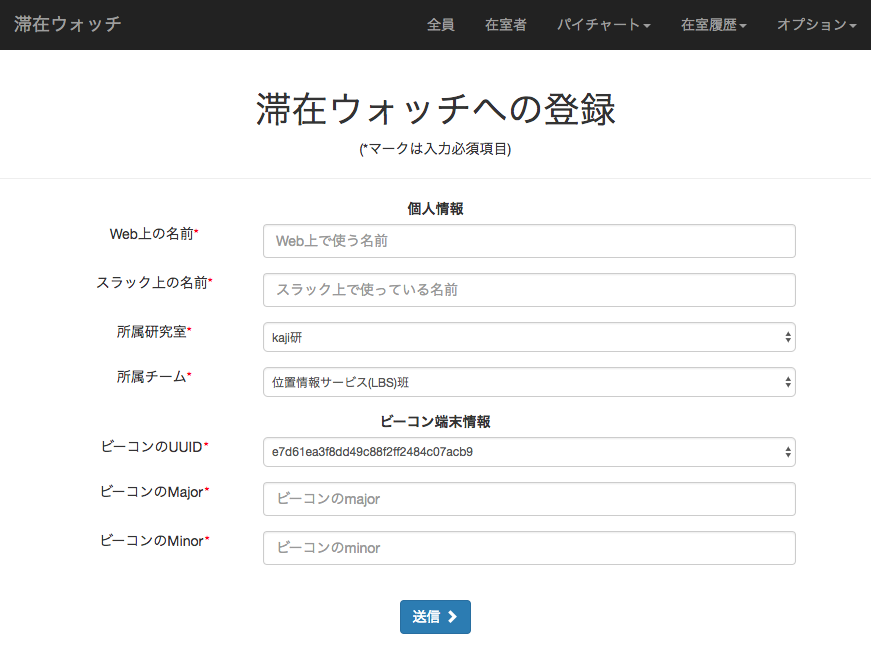
\includegraphics[width=160mm]{image/RegistrationScreen.png}
    \caption{登録画面}
    \label{fig:ent}
  \end{center}
\end{figure}

% 利用者がビーコンを携帯し部屋に訪れると,部屋ごとに設置された受信機でビーコンを検出する.
% この手法では,利用者は常にビーコンを所持している必要がある.
% FCS1301は小型で薄いビーコンのため,財布の中や鍵のキーホルダーとして貴重品などと一緒に持ち歩ける.
% この手法では,一時的に部屋を出た場合にも在室判定ができ,利用者はビーコンを所持するだけで,在室者情報を記録できる.
% 利用者が部屋を訪れた際,部屋ごとに設置された受信機で検出されたビーコンの情報とサーバにある登録情報を参照し,在室者を特定する.
% また,複数の部屋に受信機を設置する可能性があるため,在室者の名前に加えて部屋名もサーバに送信する.
% 部屋ごとに受信機を設置する際に,設置する部屋が隣接する場合に以下の問題が発生する可能性がある.
% ビーコンは周囲数メートルから数十メートルに電波を発信するため,隣接した複数の部屋で同様の在室判定を行う可能性がある.
% そこで,ビーコンが発信する電波強度に着目する.
% ビーコンの電波強度は表\ref{tb:rf}に示すように壁や扉のコンクリートや鉄板の障害物によって減衰する\cite{barrier}.
% そのため,隣接した複数の部屋では電波強度に明らかな差があると考えられる.
% したがって,在室判定にビーコンの受信電波強度を利用して隣接した部屋での誤検出の防止が可能だと考える.

% \begin{table}[H]
%   \begin{center}
%     \caption{高周波 (RF) 電波を反射/吸収する物質}
%     \label{tb:rf}
%     \begin{tabular}{|c||c|c|c|c|c|c|c|c|c|} \hline
%       障壁の種類   & 木材 & 合成物質 & ガラス & 水 & 煉瓦 & 大理石 & 土壁 & コンクリート & 金属       \\ \hline
%       干渉の可能性 & 低   & 低       & 低     & 中 & 中   & 中     & 高   & 高           & 非常に高い \\ \hline
%     \end{tabular}
%   \end{center}
% \end{table}

% 部屋ごとに設置された受信機によって検出された在室者情報はサーバに送られ,データベースに日時と在室した部屋名が記録される.
% 記録した在室者情報はWeb APIを通して利用可能であり,他のプログラムからも利用できる.
% Web APIの利用方法は指定のURLを開くとJSON形式\cite{json}で取得できる.
% 例えば,https://kajilab.net/stay-watch/stay にアクセスすると現在の在室者情報が取得できる.
% 実際に取得したJSON形式の在室者情報を図\ref{jsonstay}に示す.
% 図\ref{jsonstay}に示すように,現在在室している人のID,名前,所属,在室している部屋を取得できる.
% この他にもhttps://kajilab.net/stay-watch/ に続けてリクエストパラメータがある.
% リクエストパラメータについて表\ref{request}に示す.

% \begin{figure}[H]
%   \begin{center}
%     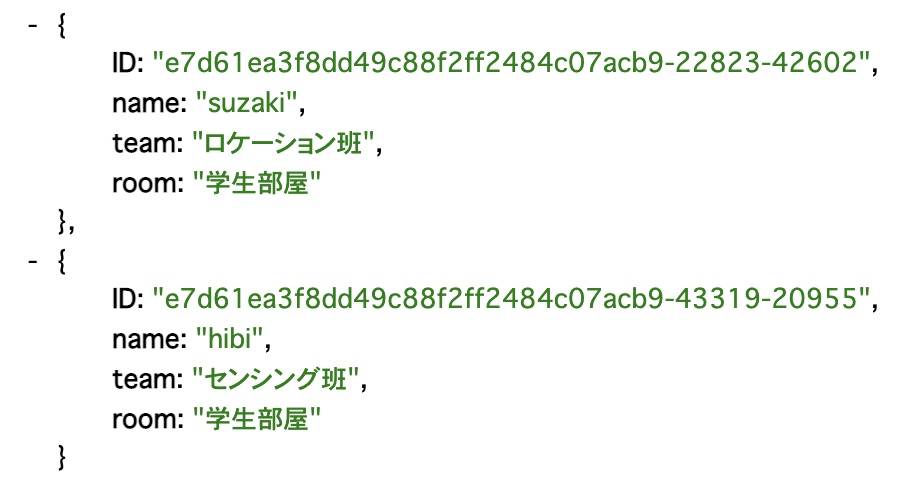
\includegraphics[width=160mm]{image/jsonstay.png}
%     \caption{JSON形式で取得した現在の在室者情報}
%     \label{jsonstay}
%   \end{center}
% \end{figure}
% \begin{table}[H]
%   \begin{center}
%     \caption{リクエストパラメータ一覧}
%     \label{request}
%     \begin{tabular}{|l|c|c|} \hline
%       パラメータ             & 値     & 説明                                       \\ \hline
%       stay                   & string & 現在の在室者を取得する                     \\ \hline
%       log                    & string & 今日の在室情報のみを取得する               \\ \hline
%       log?date1= YYYY-MM-DD
%                              & string & 過去の在室情報を取得(date1からdate2)       \\

%       \&date2=MMMM-YY-DD     &        &                                            \\\hline
%       last-time              & string & 最後に滞在を確認できた時間を取得する       \\ \hline
%       log-time               & string & 過去の累計滞在時間を取得する               \\ \hline
%       log-time?month=YYYY-MM & string & 過去の累計滞在時間を月ごとに取得する       \\ \hline
%       log-group              & stirng & その日だけのグループの滞在情報を取得する   \\ \hline
%       log-group?date1=YYYY-MM-DD
%                              & stirng & 期間を指定してグループの滞在情報を取得する \\
%       \&date2=YYYY-MM-DD     &        & (date1からdate2)                           \\\hline
%     \end{tabular}
%   \end{center}
% \end{table}